
%% ================================================================
%%  2.  RELATED WORK
%% ================================================================
\section{Related Work}\label{sec:related}

We organize the related literature into five areas: classical OR
foundations, heuristic inventory policies, reinforcement learning
for inventory management, graph neural networks for supply chains,
and---most relevant to our contribution---existing benchmarking efforts
and their limitations. \Cref{fig:timeline} provides a chronological
overview of the key milestones in both solution methods and
benchmarking infrastructure.

\begin{figure}[htbp]
  \centering
  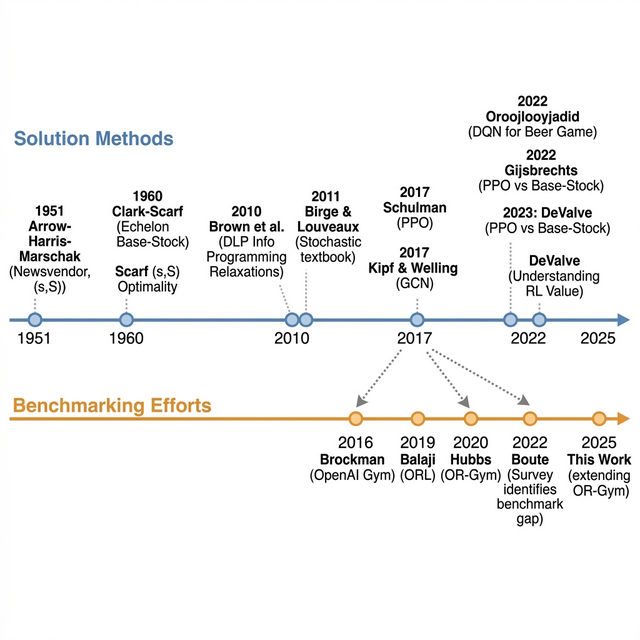
\includegraphics[width=\textwidth]{figures/literature_timeline.png}
  \caption{Timeline of key developments in inventory management methods
           (top track, blue) and benchmarking efforts (bottom track,
           orange). Dotted arrows indicate environmental framework
           dependencies. Our work (rightmost) builds upon OR-Gym
           rather than introducing a new framework.}
  \label{fig:timeline}
\end{figure}

\subsection{Classical Operations Research for Inventory Management}

The mathematical study of inventory control dates to
\citet{arrow1951optimal}, who formulated the single-period newsvendor
problem and introduced the $(s, S)$ ordering policy. \citet{scarf1960optimality}
later proved the optimality of $(s, S)$ policies under fixed ordering costs,
establishing a theoretical cornerstone of inventory theory.

For multi-echelon systems, \citet{clark1960optimal} derived optimal echelon
base-stock policies for serial networks under stationary demand---a result
that remains foundational. Extensions to tree and general network topologies
were developed by \citet{graves2000optimizing} through strategic safety
stock placement, and surveyed comprehensively by
\citet{eruguz2016comprehensive}. On the mathematical programming side,
\emph{multi-stage stochastic programming}~(MSSP) models demand uncertainty
through scenario trees~\citep{birge2011introduction}, while
\emph{deterministic linear programming}~(DLP) provides a computationally
tractable alternative by replacing uncertain demand with its conditional
expectation~\citep{brown2010information}.

These methods provide theoretically elegant solutions but share common
limitations: they require explicit distributional assumptions about demand,
their computational cost can be prohibitive for real-time applications
(particularly MSSP), and they typically assume exogenous demand---precluding
endogenous feedback mechanisms such as goodwill dynamics.

\subsection{Heuristic Inventory Policies}

Between the theoretical optimality of stochastic programming and the
data-driven flexibility of RL lie \emph{heuristic policies} that offer
practical, interpretable, and computationally cheap solutions.

The \emph{echelon base-stock policy}~\citep{clark1960optimal} decomposes
a multi-echelon network into single-node subproblems using echelon cost
accounting, with order-up-to levels derived from newsvendor critical ratios.
The $(s, S)$ \emph{reorder-point policy}~\citep{scarf1960optimality}
triggers an order when inventory falls below a threshold~$s$, bringing the
position up to target~$S$. Variations such as $(r, Q)$ fixed-quantity
policies and exponential-smoothing-based demand estimation are widely
deployed in enterprise resource planning (ERP) systems.

These heuristics are important baselines in any benchmarking study because
they represent the methods most commonly used by practitioners. A meaningful
benchmark must demonstrate whether more sophisticated (and computationally
expensive) methods provide genuine improvement over these simple but
well-tuned alternatives.

\Cref{fig:taxonomy} illustrates the four paradigms evaluated in our
benchmark and the key trade-offs between them.

\begin{figure}[htbp]
  \centering
  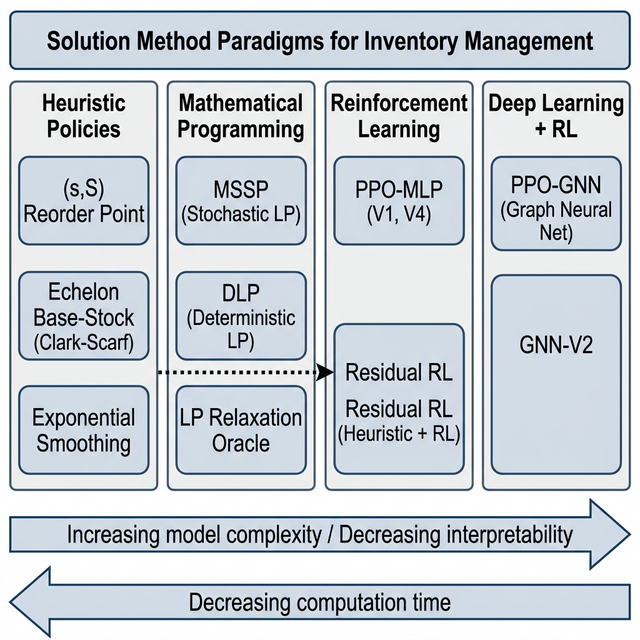
\includegraphics[width=0.85\textwidth]{figures/method_taxonomy.png}
  \caption{Taxonomy of the solution method paradigms evaluated in this
           benchmark. Methods span from interpretable, low-compute
           heuristics (left) to expressive, data-driven deep learning
           approaches (right). Residual~RL (center) bridges the
           heuristic and RL paradigms via learned corrections. The
           horizontal axes indicate two opposing trade-offs between
           interpretability and model complexity.}
  \label{fig:taxonomy}
\end{figure}

\subsection{Reinforcement Learning for Inventory Management}

The application of RL to inventory problems has gained significant momentum,
following the broader success of deep RL in sequential
decision-making~\citep{silver2016mastering}. By casting inventory
management as a Markov decision process~\citep{puterman2014markov},
RL agents can learn policies from interaction with a simulated environment
without requiring explicit demand models.

\citet{oroojlooyjadid2022deep} applied deep Q-networks~(DQN) to a
beer-game-style serial chain, demonstrating that RL can match or exceed
simple base-stock heuristics. \citet{gijsbrechts2022can} compared PPO
against base-stock policies in lost-sales and multi-echelon systems,
finding competitive performance across a range of settings.
\citet{devalve2023understanding} analysed the theoretical conditions under
which deep RL can achieve near-optimal performance, identifying problem
characteristics that favor learning-based approaches.
\citet{vanderSanden2024} conducted a simulation study comparing RL
against classical methods across different multi-echelon network
structures. \citet{meisheri2022scalable} demonstrated scalable
multi-product inventory control using RL with lead-time constraints.

A growing theme in this literature is the \emph{hybrid} approach:
combining domain knowledge with learned corrections.
The \emph{Residual RL} paradigm---where an RL agent learns additive
corrections to a base heuristic---has shown promise in leveraging the
strengths of both classical and learning-based methods. Our benchmark
includes a Residual~RL agent to evaluate this paradigm systematically.

Despite these advances, a persistent limitation is that each study
typically evaluates its RL approach on a bespoke simulation, making it
difficult to compare results across papers.

\subsection{Graph Neural Networks for Supply Chains}

Graph neural networks~(GNNs)~\citep{kipf2017semi, velivckovic2018graph}
are a natural fit for supply chain problems because the network topology is
inherently a graph. \citet{li2023gnn_sc} demonstrated GNN-based demand
forecasting for supply chain analytics, while \citet{berto2024rl4co}
explored GNN-augmented RL for combinatorial optimization problems
more broadly.

In the context of inventory management, GNNs offer a structural inductive
bias: rather than processing the supply chain state as a flat vector
(as standard MLP policies do), a GNN respects the graph topology,
enabling information to propagate along supply chain edges. Our work
is among the first to integrate a GNN as a \emph{feature extractor within
a PPO policy} for multi-echelon inventory management, and to evaluate this
architecture against both classical OR methods and standard MLP-based RL
within a controlled benchmarking framework.

\subsection{Emerging Approaches and Commercial Practice}

The most recent literature reveals a convergence of several promising
paradigms that push beyond the architectures described above.

\paragraph{Transformer-Based RL.}
\citet{tsppo2026} introduce \emph{Transformer-Sequential PPO}~(TSPPO),
which replaces graph-based feature extractors with a Transformer encoder.
Each supply chain node is treated as a token; self-attention captures
all-to-all dependencies and long-range temporal dynamics through
\emph{contextual state encoding}. While transformers excel at capturing
temporal patterns such as seasonality and trend, our experiments
(\Cref{sec:results}) show that for graph-structured supply chains, MPNN-based
GNN extractors achieve comparable performance, suggesting that the spatial
inductive bias of GNNs compensates for their lack of global attention.

\paragraph{Multi-Agent Reinforcement Learning.}
IMARL~\citep{imarl2025} combines GNNs with multi-agent learning to handle
large-scale networks by assigning each node its own policy that communicates
through the graph structure. EXPRESS~\citep{express2026} exploits structural
symmetry in multi-echelon systems to keep multi-agent models compact and
scalable. PI-PPO~\citep{pippo2026} enhances PPO convergence when managing
multiple product lines simultaneously. These approaches address the
\emph{curse of dimensionality} that occurs as network size grows---a challenge
our single-agent GNN also mitigates through its graph-structured
feature extractor.

\paragraph{Imitation Learning.}
Rather than learning purely from reward signals, \emph{behavioral cloning}~(BC)
and \emph{DAgger}~\citep{ross2011reduction} train policies to mimic expert
demonstrations. In supply chain settings, the ``expert'' can be an OR-based
oracle solver. BC provides a strong warm start but suffers from
\emph{distribution shift}: the learned policy visits states not seen in the
expert's demonstrations, leading to compounding errors. DAgger addresses this
by iteratively rolling out the current policy and querying the expert for
corrective actions, aggregating new data at each round. Our benchmark
includes both BC-initialized (GNN-IL) and DAgger-trained agents to
evaluate this paradigm.

\paragraph{Commercial State of the Art.}
In industry, several proprietary approaches have emerged that, while not
fully open, signal the direction of commercial practice.
Lokad's \emph{stochastic discrete descent}~\citep{lokad2024} operates in
``strategy space,'' evaluating financial outcomes across probabilistic
scenarios---conceptually similar to MSSP but optimized for rapid
re-computation. Kinaxis's \emph{Wahupa MEIO} engine manages non-normal
distributions across product mixes and production stages.
ToolsGroup's \emph{SO99+} uses pure probabilistic forecasting to handle
intermittent, long-tail demand at the SKU-location level.
These commercial systems highlight the practical importance of handling
distributional uncertainty---a capability our benchmark evaluates through
composable demand scenarios.

\subsection{Solution Taxonomy}\label{sec:taxonomy}

\Cref{tab:solution_taxonomy} provides a structured comparison of the
solution paradigms evaluated in this work. The key differentiator across
approaches is \emph{information access}: optimization-based methods
(Oracle, MSSP) leverage explicit demand knowledge, while RL and
imitation learning agents must infer demand dynamics from historical
observations. This information gap is the primary driver of the
performance differences reported in \Cref{sec:results}.

\begin{table}[htbp]
\centering
\caption{Taxonomy of solution approaches by architecture, information access,
and training paradigm. \emph{Future demand} refers to whether the method
has access to demand realizations beyond the current period.}
\label{tab:solution_taxonomy}
\small
\begin{tabular}{llccc}
\toprule
\textbf{Agent} & \textbf{Architecture} & \textbf{Future} & \textbf{Graph} & \textbf{Training} \\
               &                       & \textbf{Demand} & \textbf{Aware} & \textbf{Paradigm} \\
\midrule
Oracle         & LP solver             & Perfect  & \cmark & None \\
MSSP           & Stochastic LP         & Sampled  & \cmark & None \\
DLP            & Deterministic LP      & Expected & \cmark & None \\
Heuristic      & Analytical formula    & None     & Partial & None \\
$(s,S)$ Policy & Reorder-point rule    & None     & \xmark & None \\
\midrule
GNN (PPO)      & MPNN + MLP            & None     & \cmark & RL \\
TSPPO          & Transformer + MLP     & None     & Positional & RL \\
Residual RL    & Heuristic + MLP       & None     & \xmark & RL \\
\midrule
GNN-IL (BC)    & MPNN + MLP            & None     & \cmark & Imitation \\
GNN-DAgger     & MPNN + MLP            & None     & \cmark & Iterative IL \\
\bottomrule
\end{tabular}
\end{table}

Two observations are noteworthy. First, the \emph{imitation learning}
agents (GNN-IL, GNN-DAgger) use the same architecture as the RL-trained
GNN but achieve measurably higher performance by leveraging Oracle
demonstrations during training---even though at inference time they
observe exactly the same state as the RL agents and have no access to
future demand. Second, the graph-aware methods (GNN, MSSP, DLP) consistently
outperform their graph-unaware counterparts (Residual~RL, Heuristic) on
complex network topologies, validating the importance of structural
inductive biases.

\subsection{Benchmarking Efforts and the Fragmentation Problem}

The need for standardized benchmarks in inventory management has been
recognized but inadequately addressed. \citet{boute2022deep_rl_survey}
identify the lack of common evaluation infrastructure as a key barrier
to progress in deep RL for inventory control, noting that the absence
of standardized benchmarks makes it difficult to draw general conclusions.

Several efforts have attempted to fill this gap:

\begin{itemize}
  \item \textbf{OpenAI~Gym / Gymnasium}~\citep{brockman2016openai}.
        The Gymnasium framework (formerly OpenAI~Gym) established a
        standardized API for RL environments that has been transformative
        in other domains. Benchmark suites such as Atari and MuJoCo
        became the common ground upon which the RL community evaluates
        algorithmic progress. However, no comparable standard has emerged
        for inventory management.

  \item \textbf{ORL}~\citep{balaji2019orl}. Amazon's ORL project
        introduced RL benchmarks for online stochastic optimization
        problems including the newsvendor. While valuable, it focused
        on single-period problems and did not address multi-echelon
        settings or classical OR baselines.

  \item \textbf{OR-Gym}~\citep{hubbs2020orgym}. The closest predecessor
        to our work, OR-Gym provides Gymnasium-compatible environments
        for several OR problems including multi-echelon inventory
        management. However, OR-Gym was limited to stationary demand,
        a single RL algorithm, and did not implement OR-based
        solution methods for comparison.
\end{itemize}

A common pattern across these efforts is that they are \textbf{not
cumulative}: each introduces a new framework rather than extending a
previous one. Subsequent researchers typically develop yet another bespoke
environment tailored to their specific contribution, rather than building
upon these existing platforms. This fragmentation means that results
across studies are not directly comparable---different cost structures,
demand models, episode lengths, and performance metrics make apples-to-apples
evaluation impossible.

Our work takes a deliberately different approach. Rather than creating
another environment from scratch, we \textbf{build upon and extend} the
OR-Gym framework---modernizing it to the current Gymnasium~API, adding
composable non-stationary demand, endogenous goodwill dynamics, and
critically, implementing classical OR solution methods (MSSP, DLP,
echelon base-stock, $(s, S)$) as first-class agents within the same
framework. This enables cross-paradigm evaluation on identical scenarios
with identical metrics for the first time.

\Cref{tab:benchmark_comparison} summarizes how our framework compares
to prior benchmarking efforts.

\begin{table}[htbp]
\centering
\caption{Comparison of inventory management benchmarking efforts.}
\label{tab:benchmark_comparison}
\small
\begin{tabular}{lcccc}
\toprule
\textbf{Feature} & \textbf{ORL} & \textbf{OR-Gym}
                  & \textbf{Ours} \\
\midrule
Multi-echelon topologies     & \xmark & \cmark & \cmark \\
Non-stationary demand        & \xmark & \xmark & \cmark \\
Endogenous dynamics          & \xmark & \xmark & \cmark \\
Classical OR agents          & \xmark & \xmark & \cmark \\
Multiple RL architectures    & \xmark & \xmark & \cmark \\
GNN-based agents             & \xmark & \xmark & \cmark \\
Formal metrics (VPI/VSS)     & \xmark & \xmark & \cmark \\
Statistical testing          & \xmark & \xmark & \cmark \\
Current Gymnasium API        & \xmark & \xmark & \cmark \\
Open-source                  & \cmark & \cmark & \cmark \\
\bottomrule
\end{tabular}
\end{table}
